\chapter{Steam Software User Interface and Task Explanation}
\section{Figures associated with the Steam Store}
\begin{figure}[H]
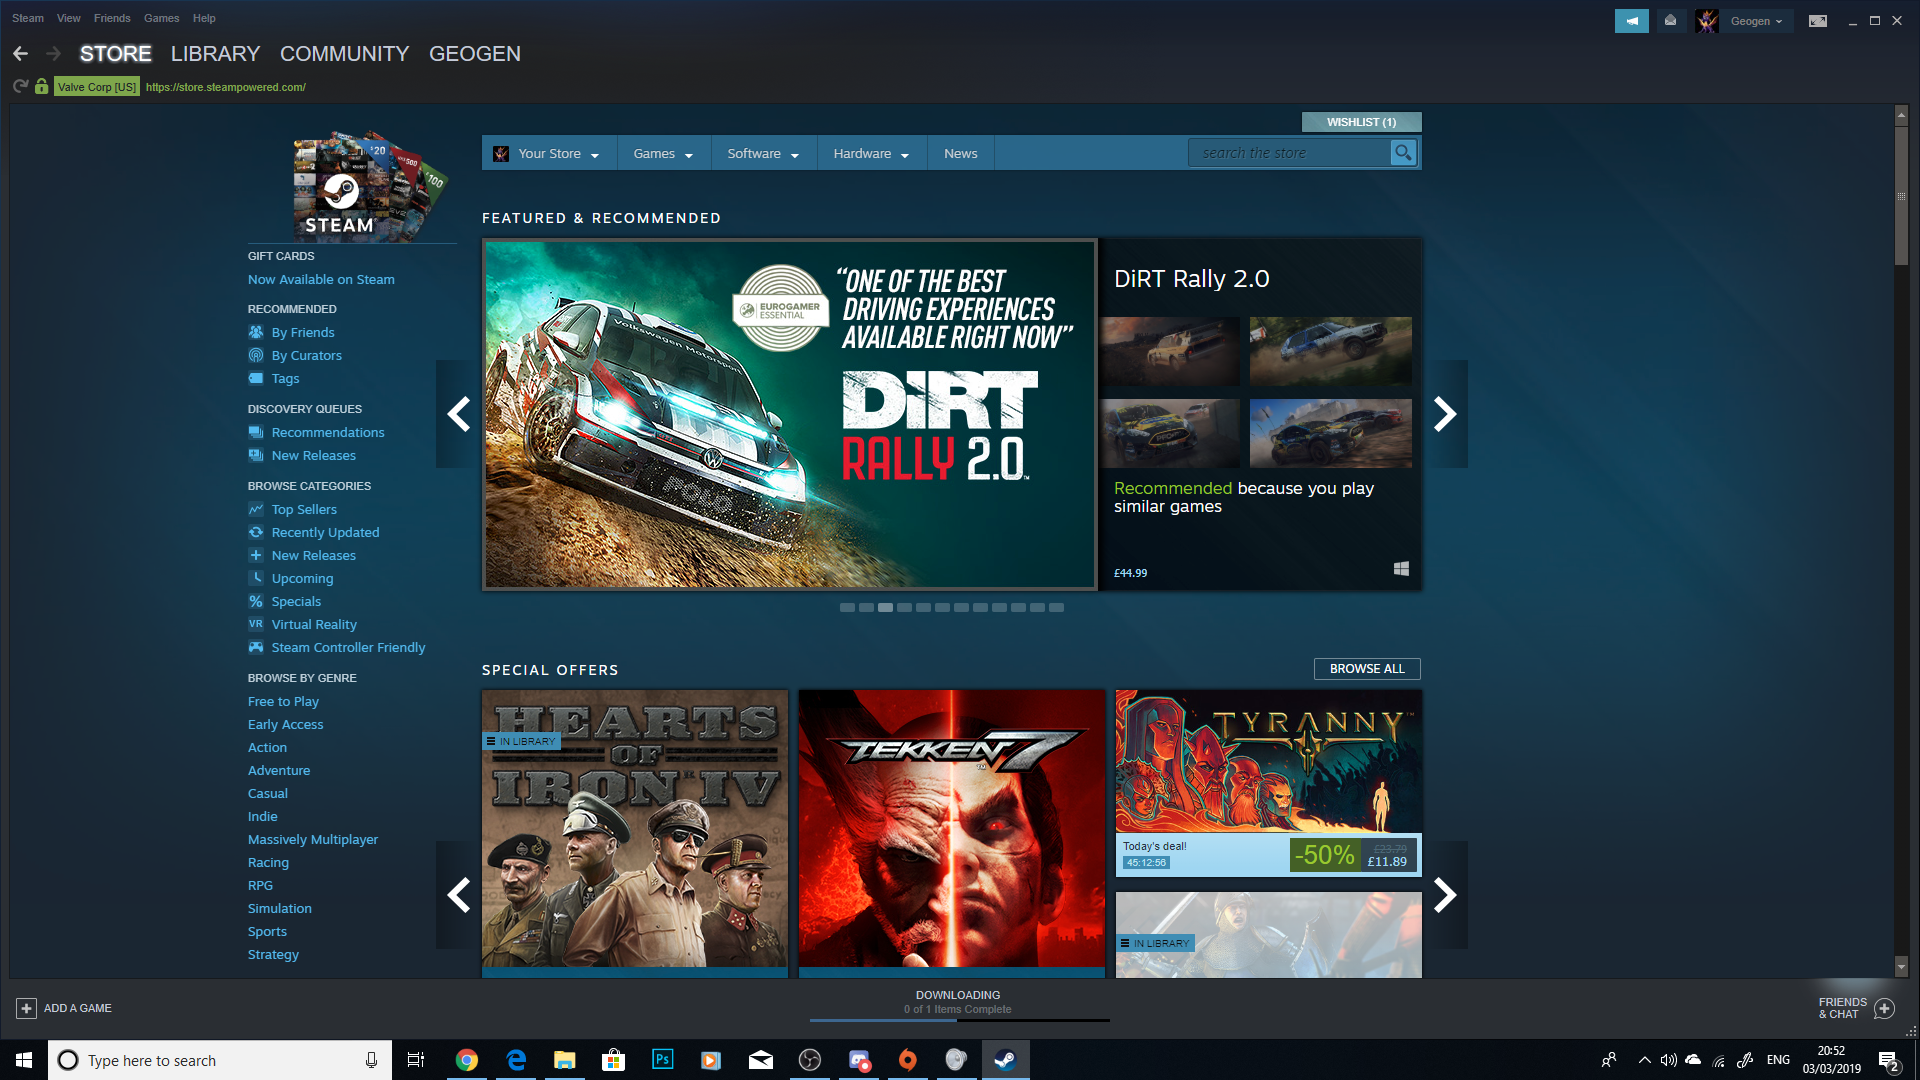
\includegraphics[width=16cm,height=9cm]{Screenshots/SteamScreenShots/SteamMainShopMenu.png}
\caption{Steam Client Store Menu}	
\end{figure}
This is the default page for Steam and what would greet the user upon logging in. It displays the available games for purchase, with sub-categories available from the left hand side. There are a great number of interactive elements on this screen, so it may take some time for study participants to find exactly what they are looking for.

\begin{figure}[H]
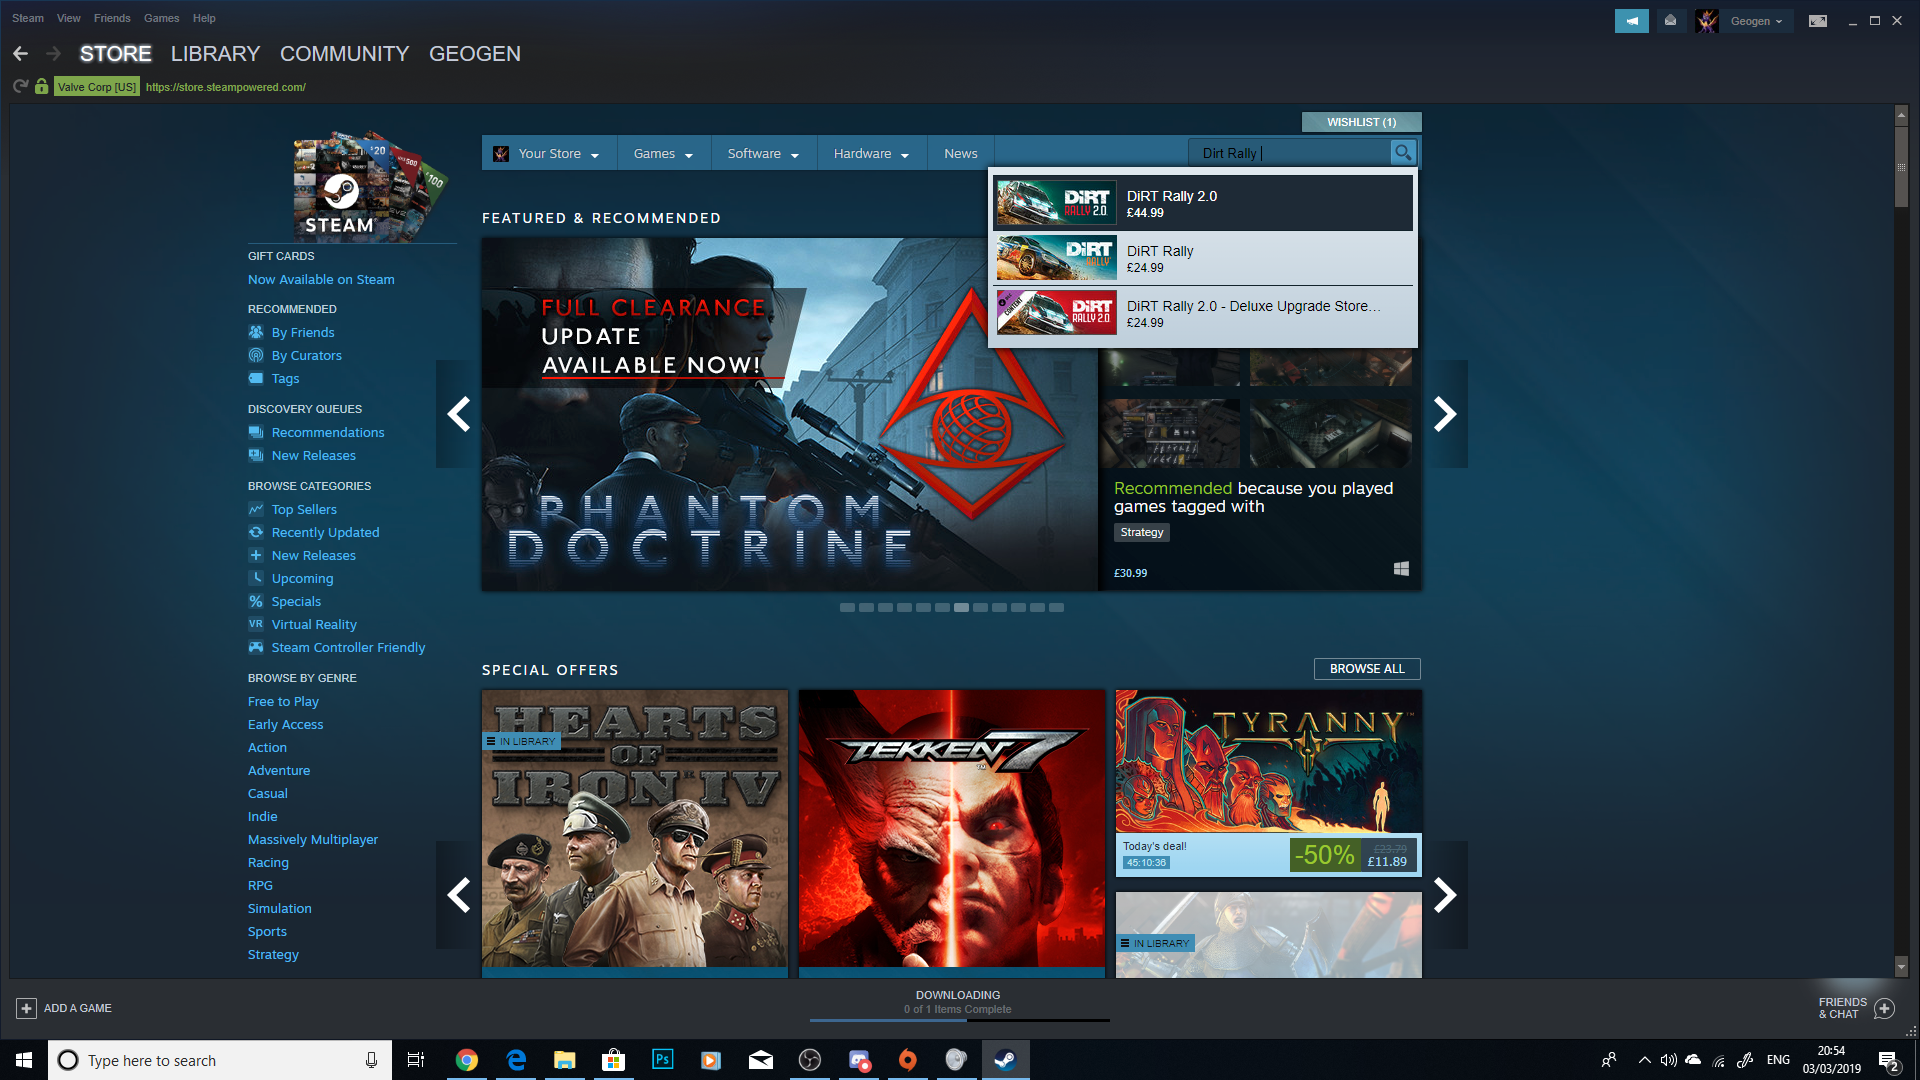
\includegraphics[width=16cm,height=9cm]{Screenshots/SteamScreenShots/SearchingForAGame.png}
\caption{Searching for a title "DIRT 2.0" on the Steam Store Page}
\end{figure}
The above Figure demonstrates the basic search functionality of the Steam Store, where a user would type in the name of a specific game, or secondly an associated word such as a games publisher like "Codemasters" for the "Dirt Rally" franchise. Upon clicking a certain title, a page similar to Figure 4 shall appear.

\begin{figure}[H]
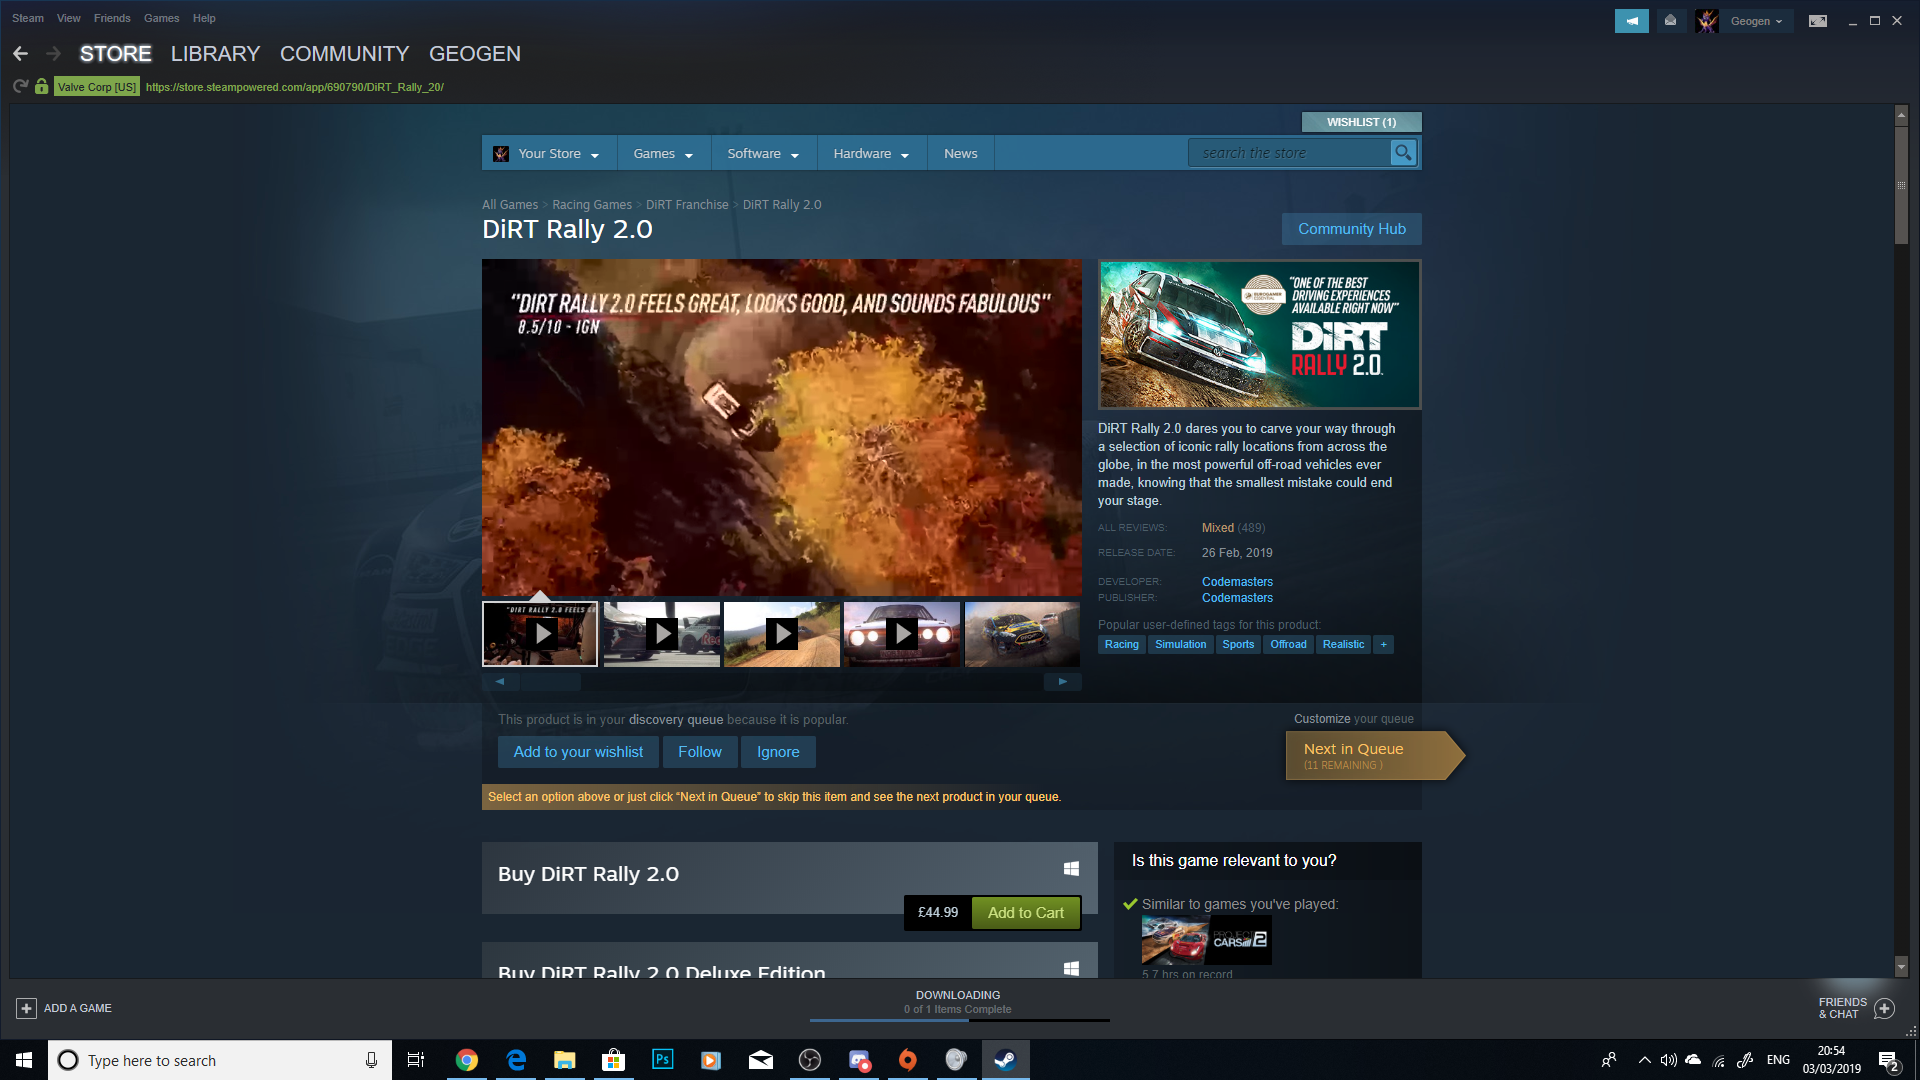
\includegraphics[width=16cm,height=9cm]{Screenshots/SteamScreenShots/PageForSearchedGameDirt.png}
\caption{Store Page for Searched Title - ``DIRT Rally 2.0"}    
\end{figure}
This page shows information about the searched title "DIRT Rally 2.0", the user can view the games description, any media such as video trailers and screen-shots from the game, they can choose to purchase the game, view overall community reception to the game, among other functions.

\section{Figures associated with the Steam Library - Installing a Game}
\begin{figure}[H]
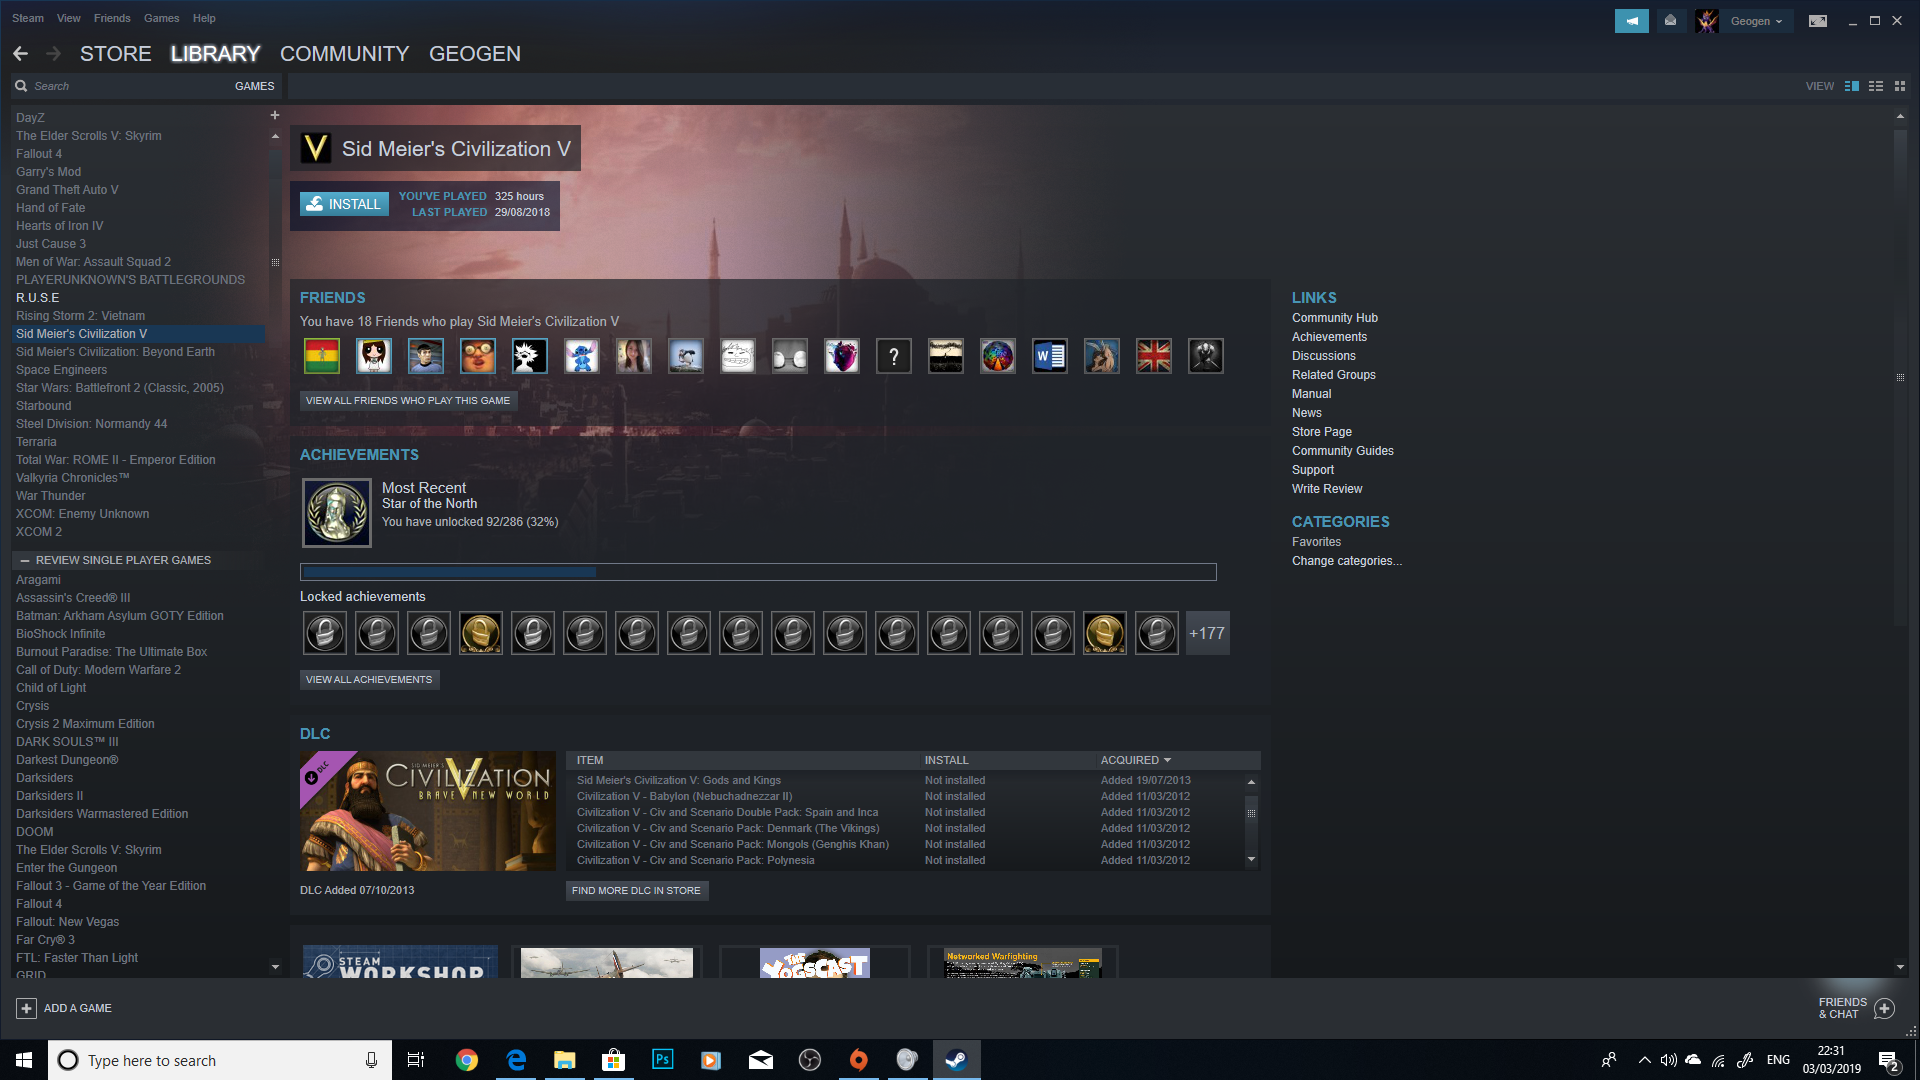
\includegraphics[width=16cm,height=9cm]{Screenshots/SteamScreenShots/SelectAPurchasedGame.png}
\caption{Selection of ``Sid Meier's Civilization 5" in the purchased Library of Games}    
\end{figure}
This is the Steam library page, on the left hand side are a series of game titles belonging to my account. To install a title, a user would right click the desired game, and then follow the dialog box then is displayed in Figure 6.

\begin{figure}[H]
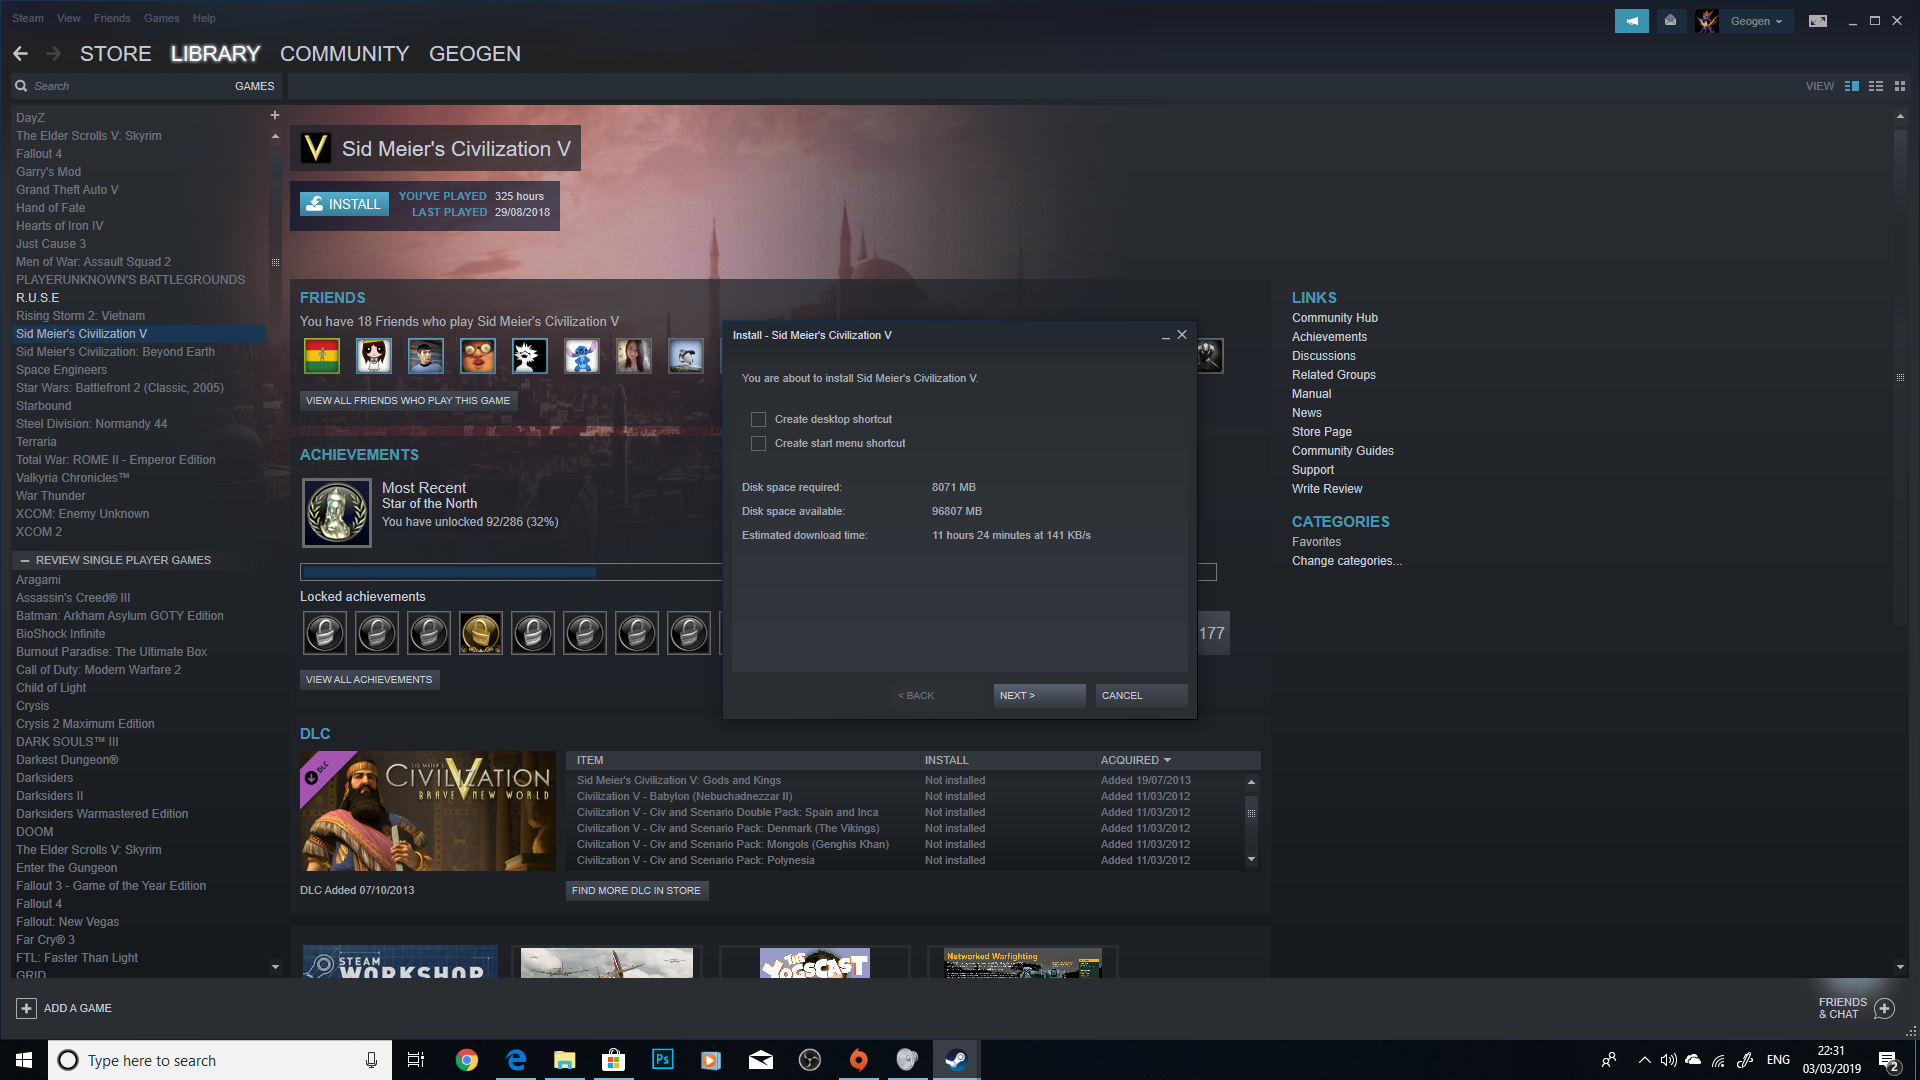
\includegraphics[width=16cm,height=9cm]{Screenshots/SteamScreenShots/InstallDialogForCivilisation5.png}
\caption{Installation Dialog Message Box - Sid Meier's Civilization 5}    
\end{figure}
The dialog box gives users information on what game they are installing and data such as installation size and the set file path. 

\section{Figures associated with Steam Community Modifications of Sid Meier's Civilization 5}

\begin{figure}[H]
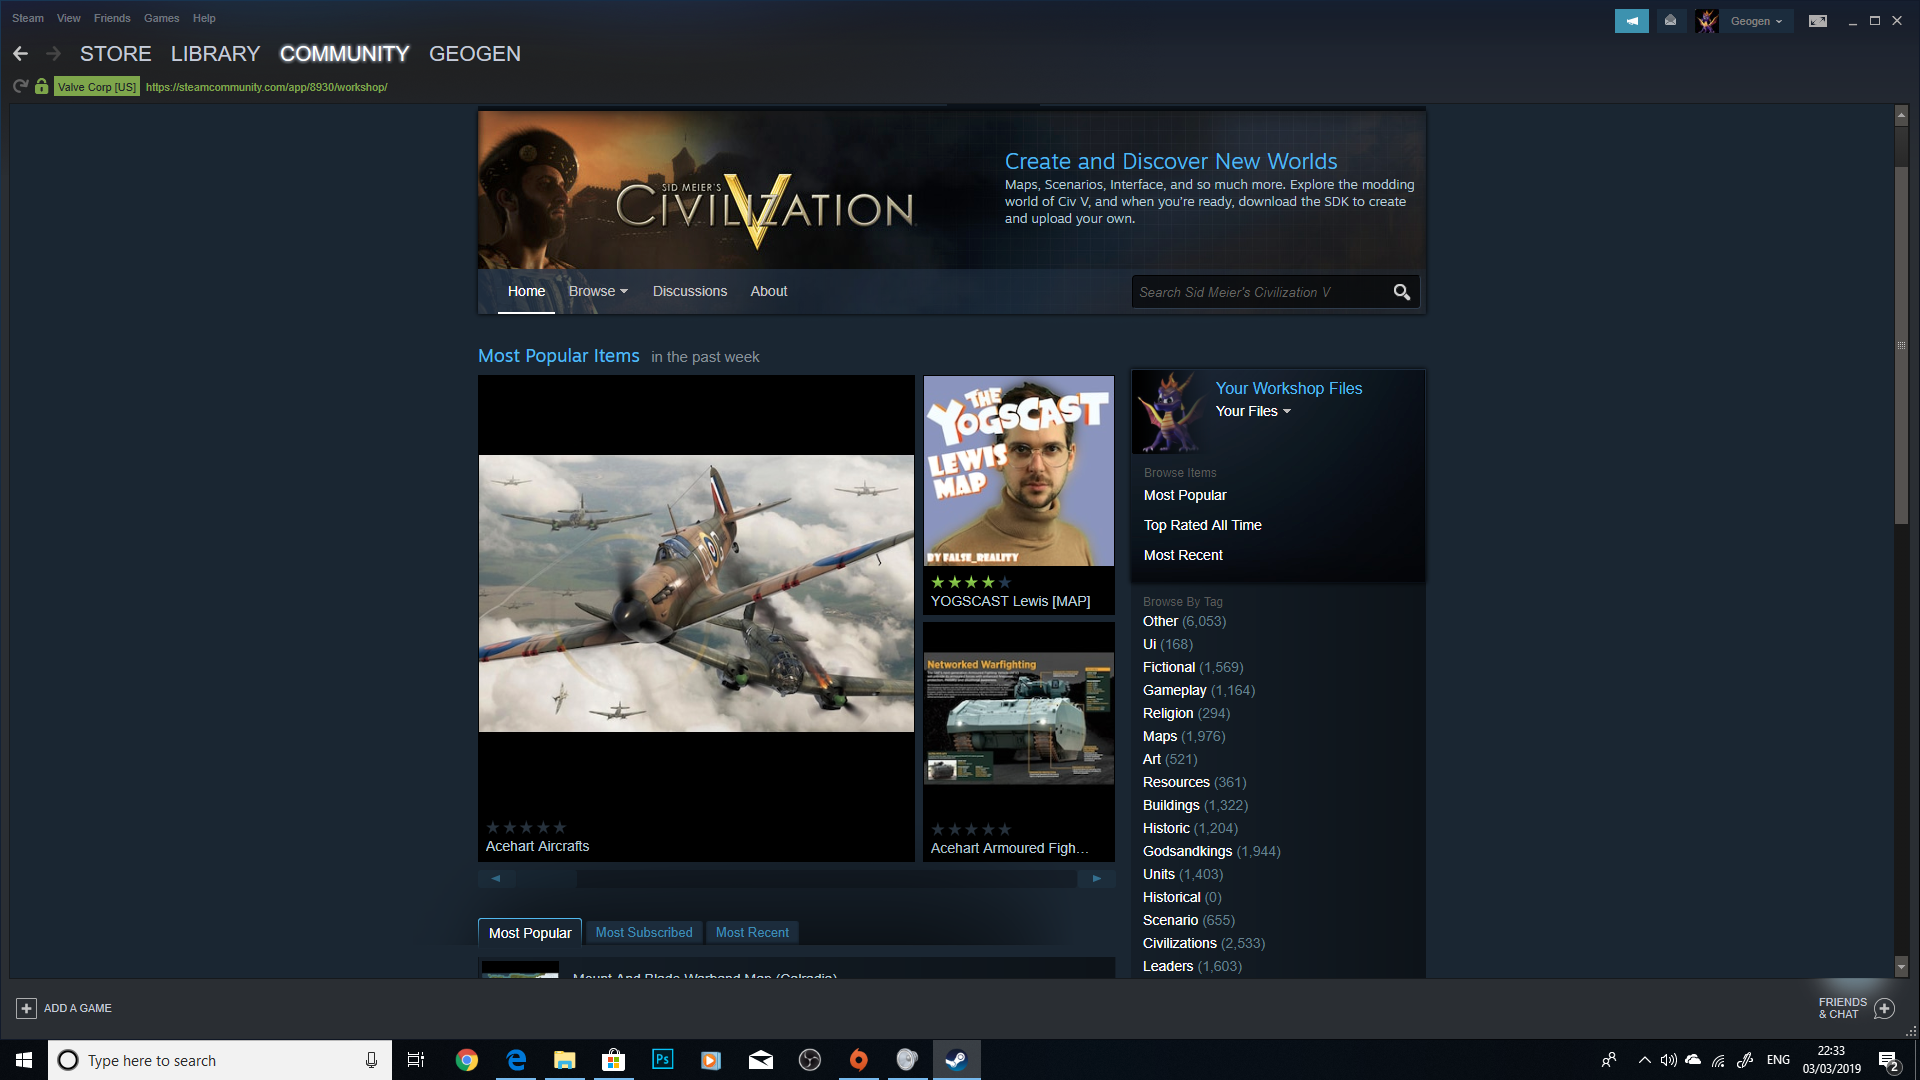
\includegraphics[width=16cm,height=9cm]{Screenshots/SteamScreenShots/CommunityForCivilisation5.png}
\caption{Community Section for Sid Meier's Civilization 5}    
\end{figure}

This is the community section of the Steam client, it is used for a number of functions, including that of finding modifications for certain games, such as Sid Meier's Civilization 5. The user can find modifications suited to what they want to change, for instance music or graphical elements. For ease of use, many users would be interested in the most popular mods, which this UI offers as a shortcut seen at the centre - bottom of the image. 

\begin{figure}[H]
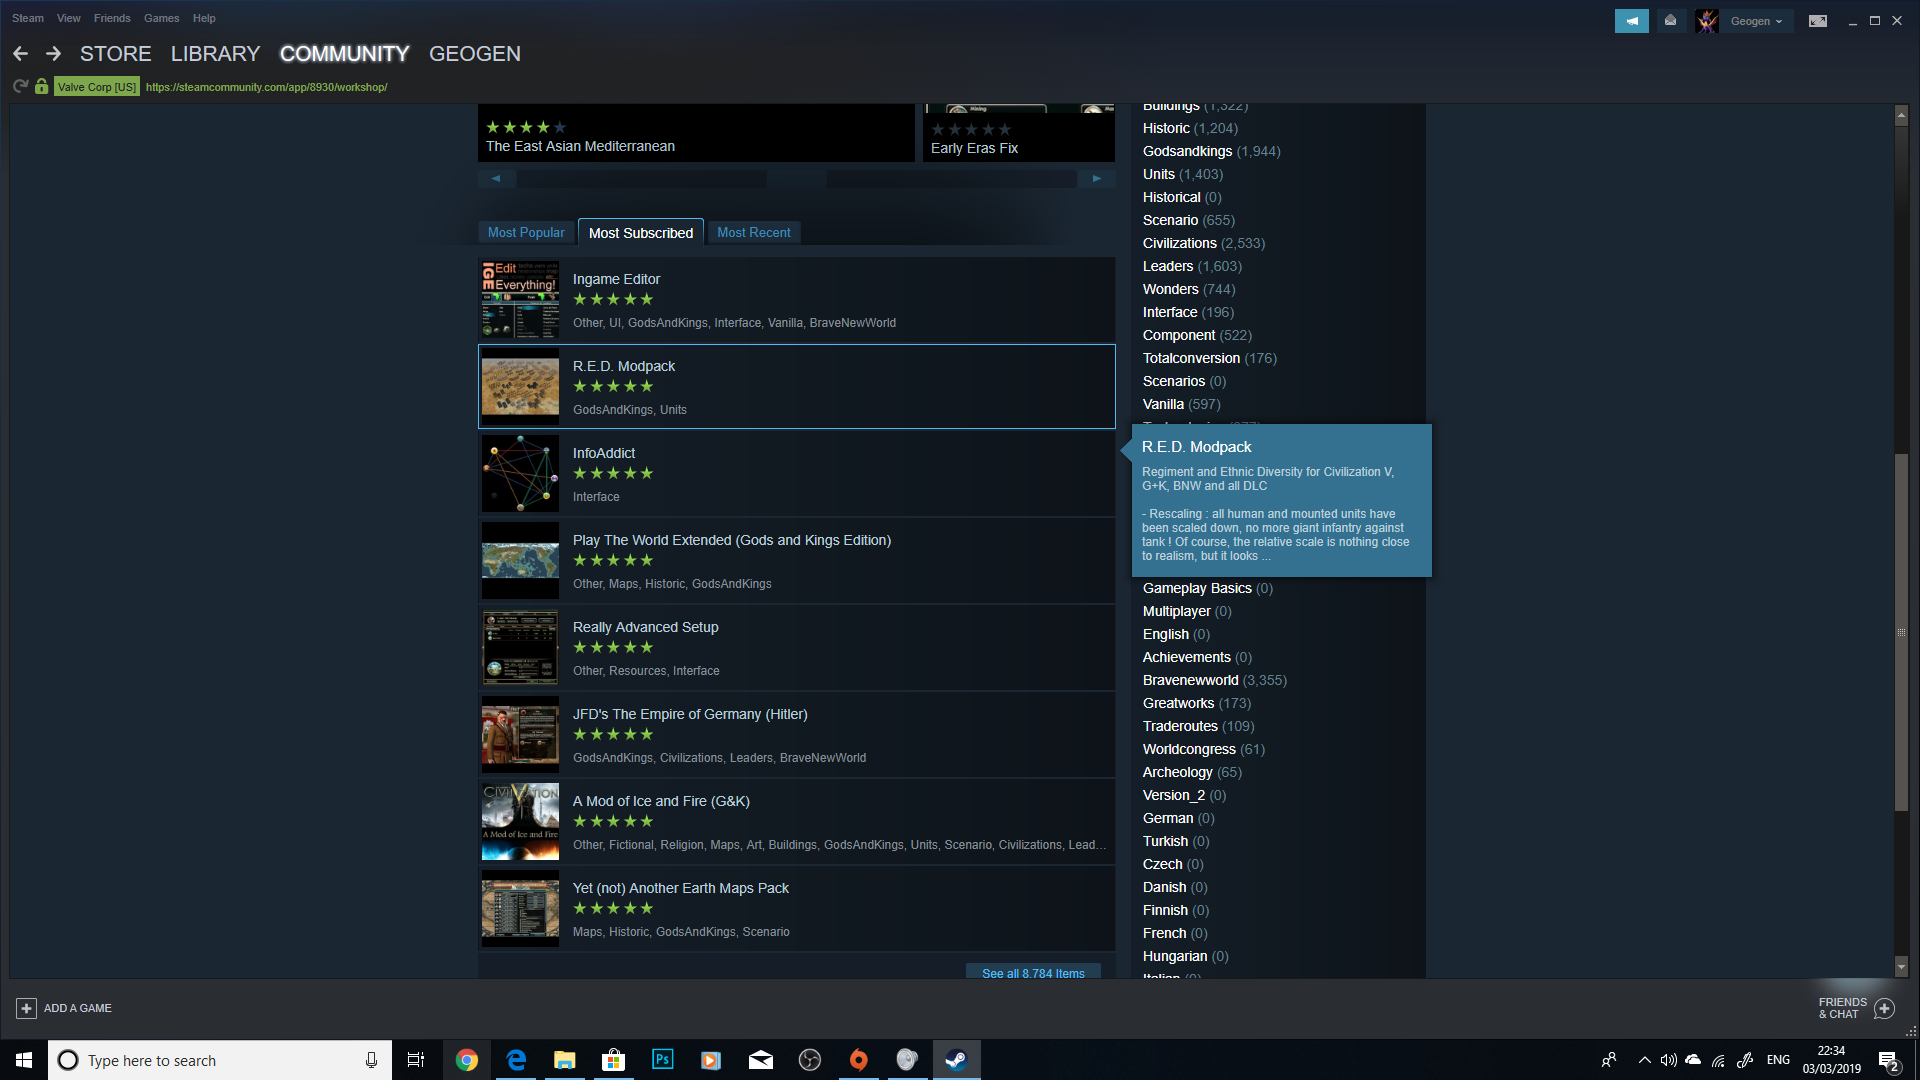
\includegraphics[width=16cm,height=9cm]{Screenshots/SteamScreenShots/FindingAModForCivilisation5.png}
\caption{Finding a Modification for Sid Meier's Civilization 5}    
\end{figure}

Once the user has clicked on the "Most Subscribed" element, a list of the most popular modifications is presented for the user to browse.

\begin{figure}[H]
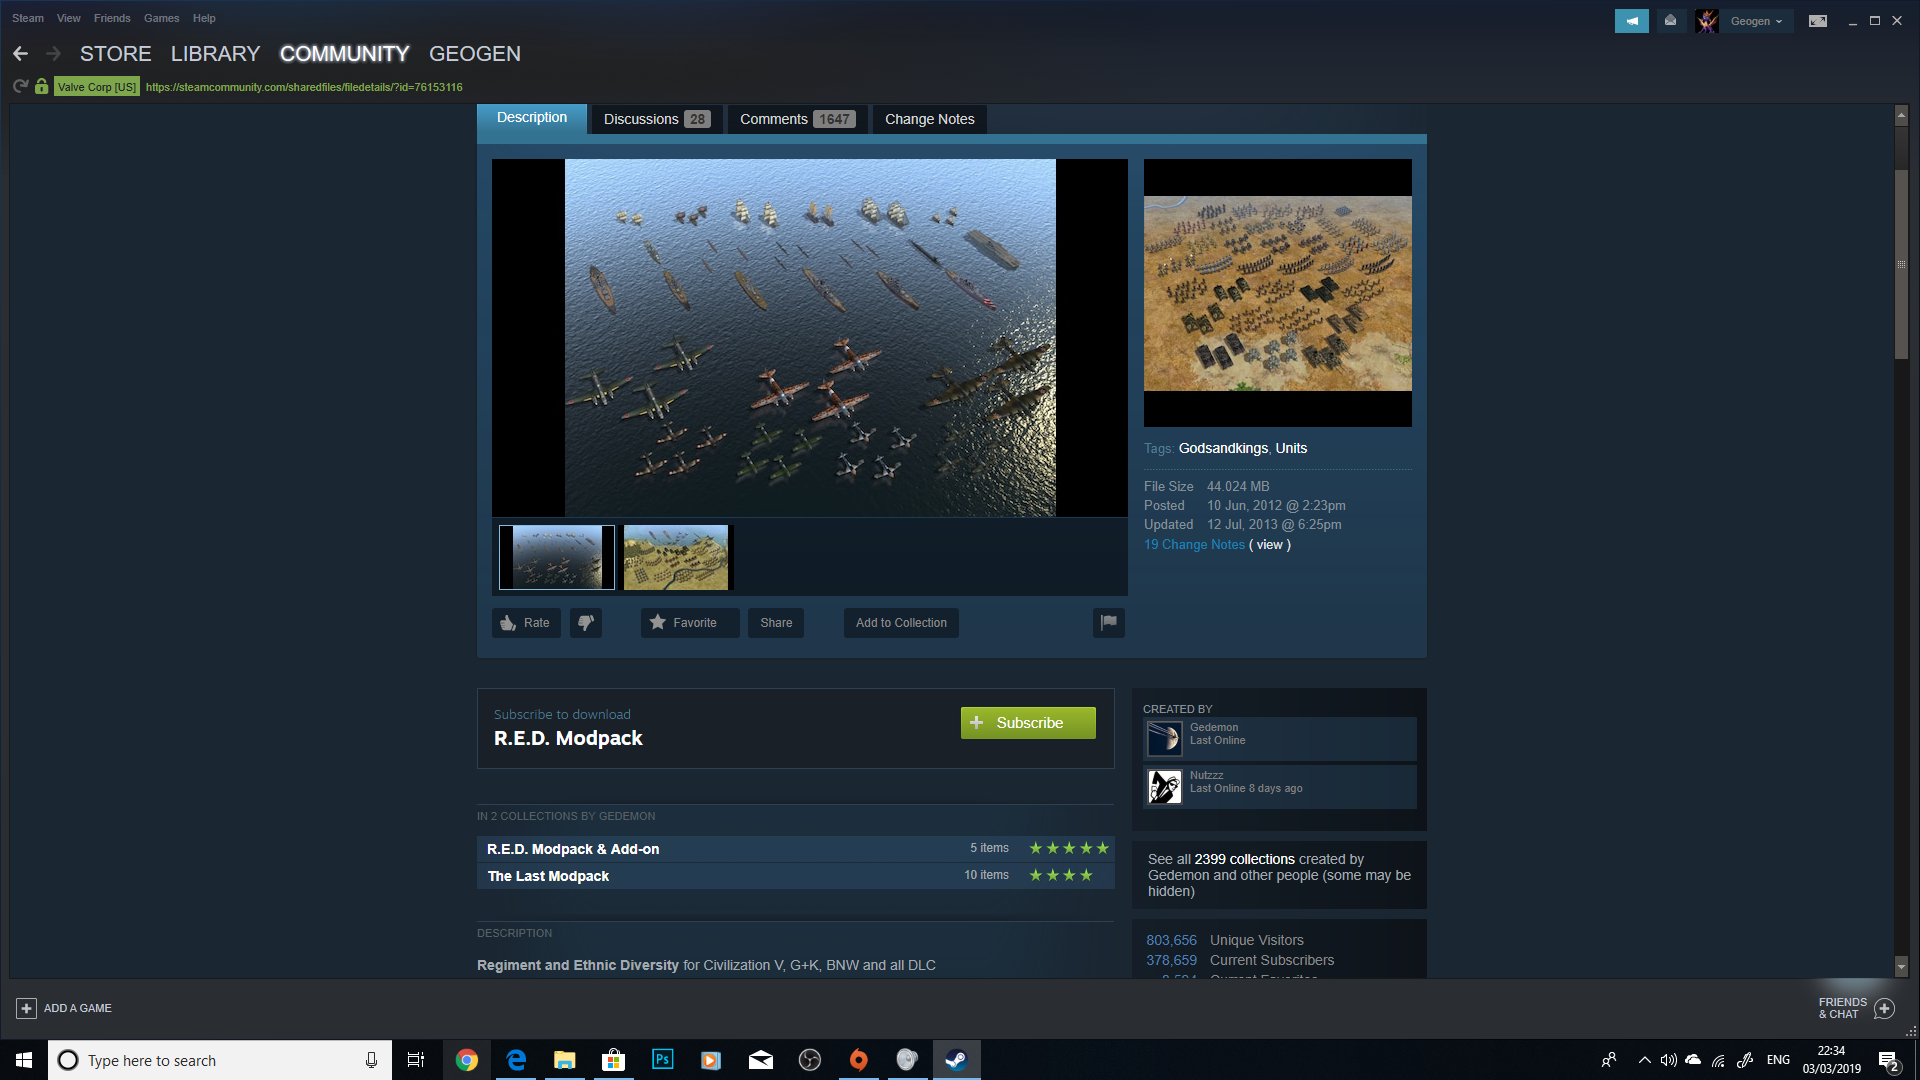
\includegraphics[width=16cm,height=9cm]{Screenshots/SteamScreenShots/SubscribingToSelectedMod.png}
\caption{Subscribing to the R.E.D Modpack for Sid Meier's Civilization 5}    
\end{figure}

Upon clicking a particular modification of interest, the user is brought to a page detailing what the mod is, and the ability to ``subscribe to the mod". 

\section{Figures associated with verifying an installed game}

\begin{figure}[H]
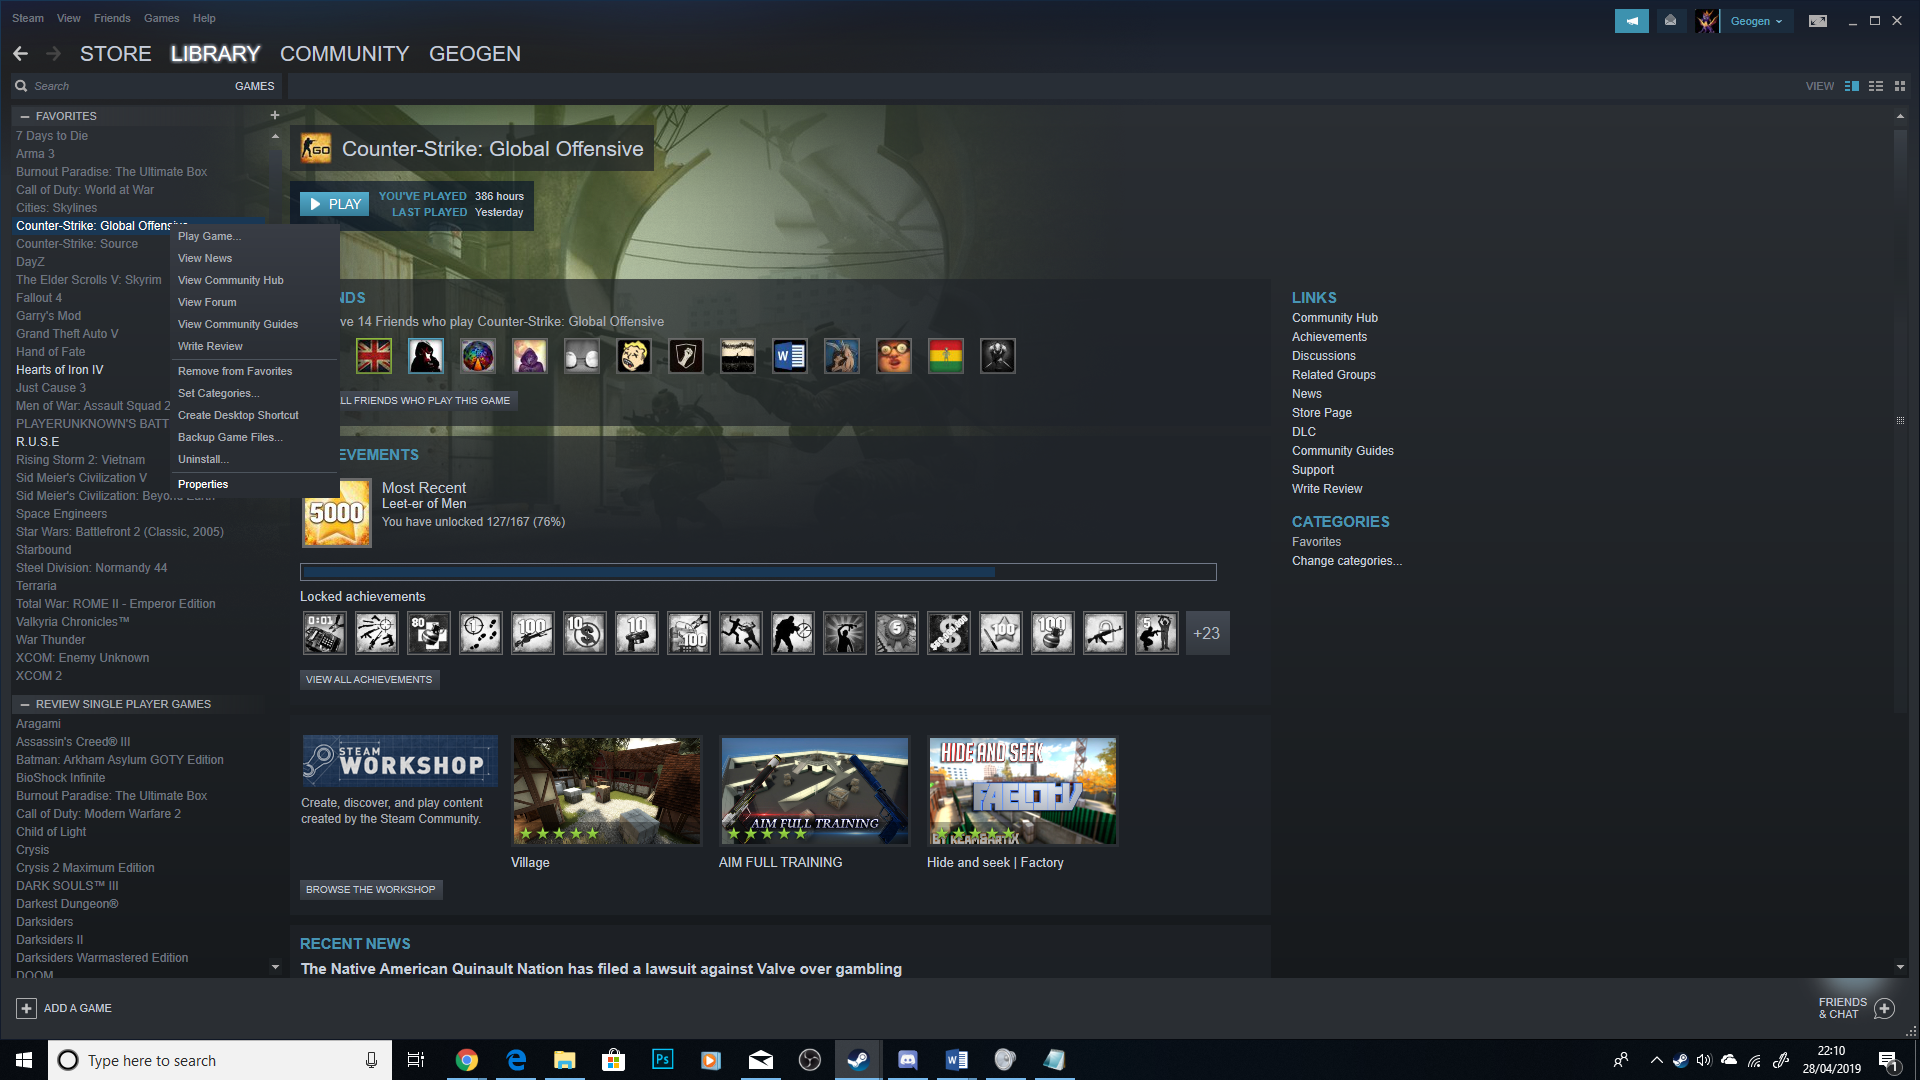
\includegraphics[width=16cm,height=9cm]{Screenshots/SteamScreenShots/verifyCSProperties.png}
\caption{Opening a selected game properties menu from Steam Library page}    
\end{figure} 

This Figure shows an installed game ``Counter-Strike Global Offensive", I have right clicked on the white text to bring up a new menu, I am about to click on properties to bring up further options for this particular game.

\begin{figure}[H]
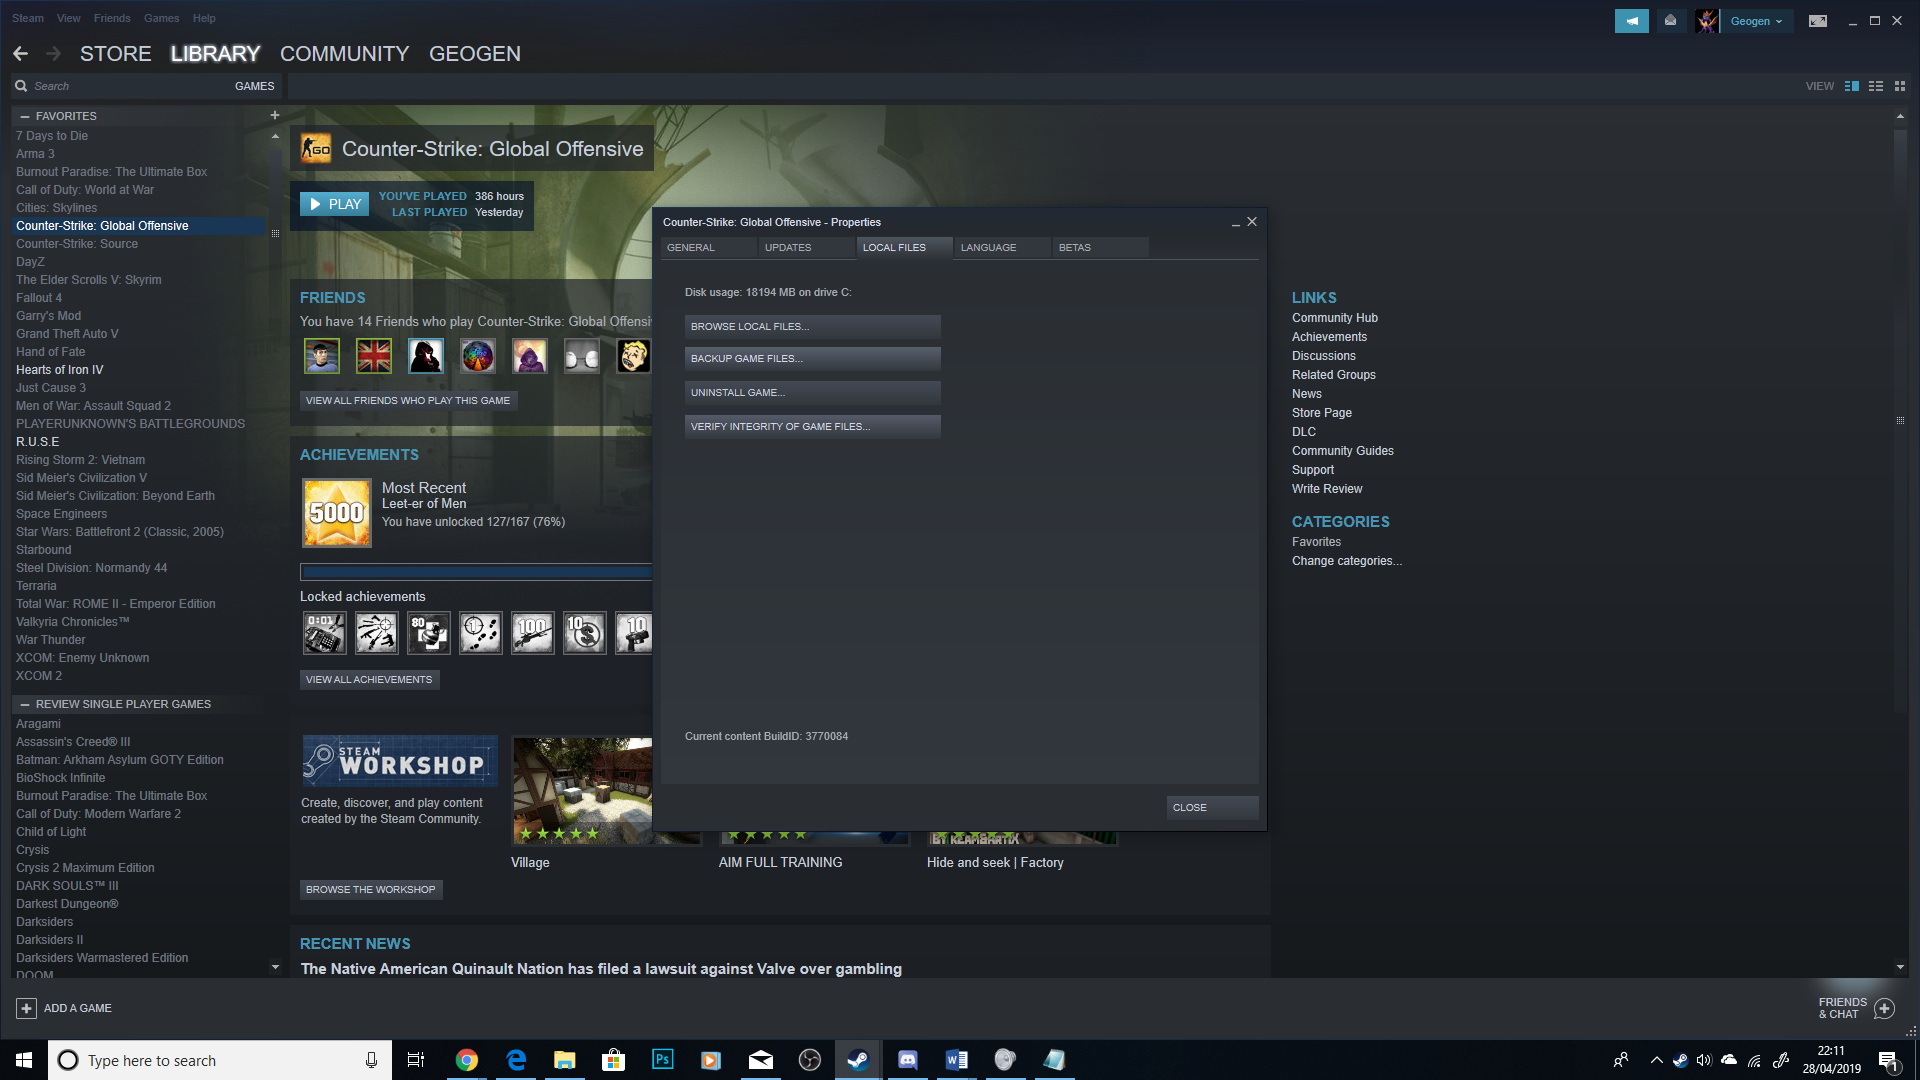
\includegraphics[width=16cm,height=9cm]{Screenshots/SteamScreenShots/verifyCSButtonLocation.png}
\caption{Locating the Verification of game files button for Counter-Strike : Global Offensive}    
\end{figure} 

I have located the required button to verify the game installed game files for Counter Strike : Global Offensive , \textit{``Verify Integrity of Game Files"}. 

\begin{figure}[H]
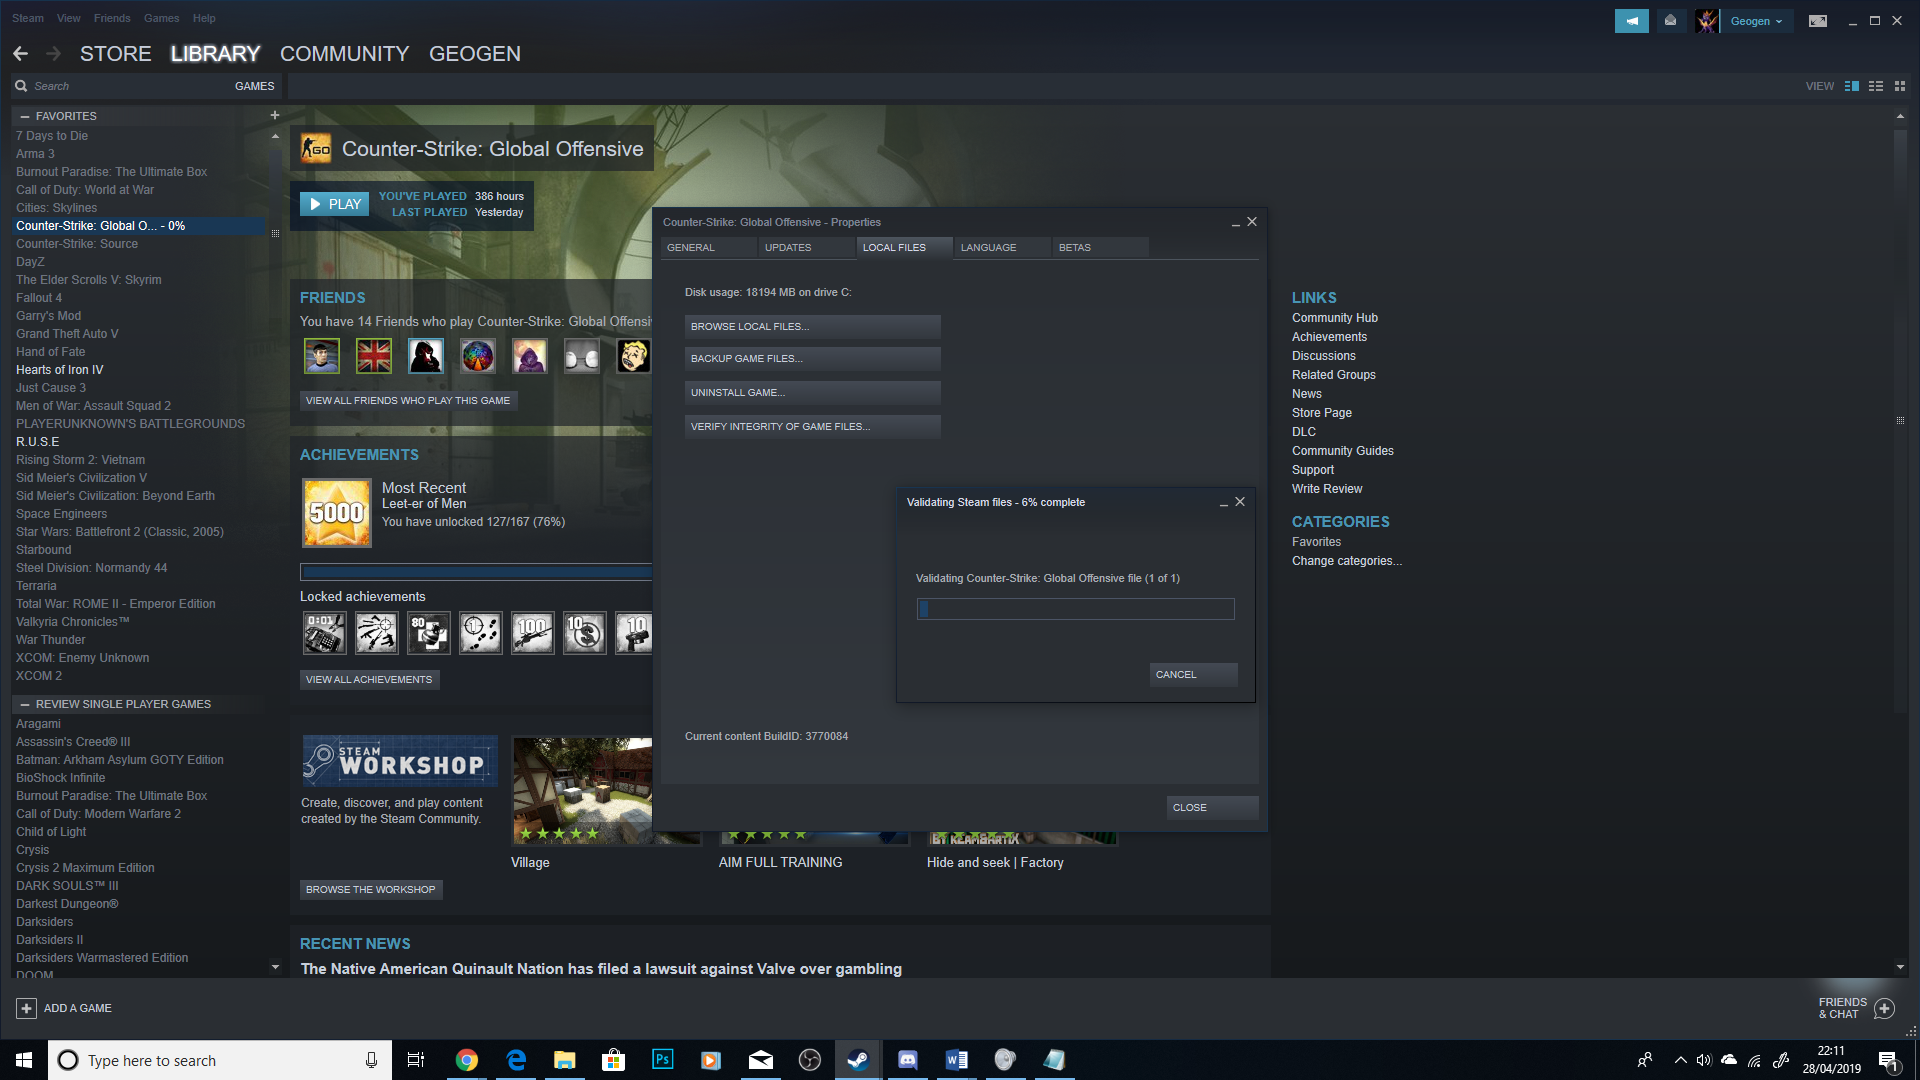
\includegraphics[width=16cm,height=9cm]{Screenshots/SteamScreenShots/verifyProcess.png}
\caption{Locating the Verification of game files button for Counter-Strike : Global Offensive}    
\end{figure}

I have clicked upon the desired button element, and the verification process has begun.

\section{Figures associated with the Big Picture Mode}
\begin{figure}[H]
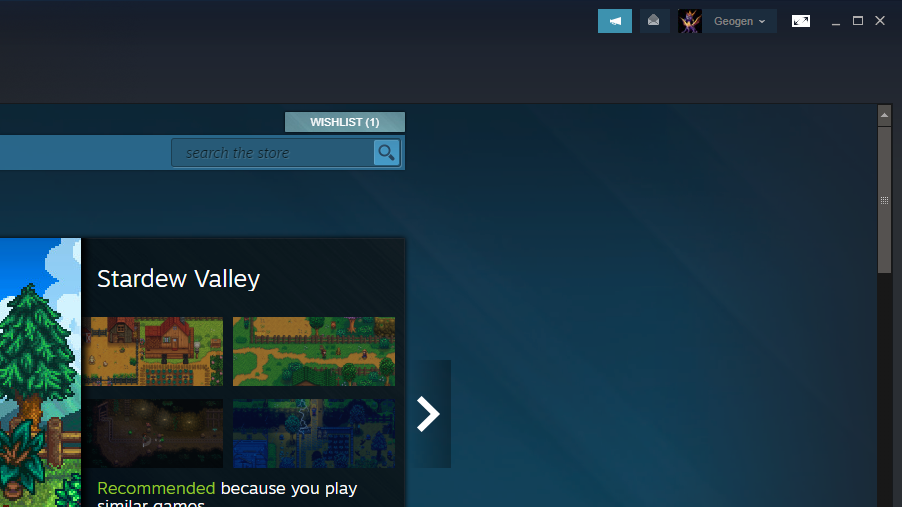
\includegraphics[width=16cm,height=9cm]{Screenshots/SteamScreenShots/BigPictureModeTopRightCropped.png}
\caption{Location of Steams Big Picture Mode}    
\end{figure} 

This image, although similar to the image in Figure 2. This image focuses on the location of the UI element to change the Steam interface into big picture mode, it is located at the top right hand side of the client, near the user-name and user picture. It is indicated by a white rectangle with arrows. The interface will change to what is pictured in Figure 10, upon clicking the box.

\begin{figure}[H]
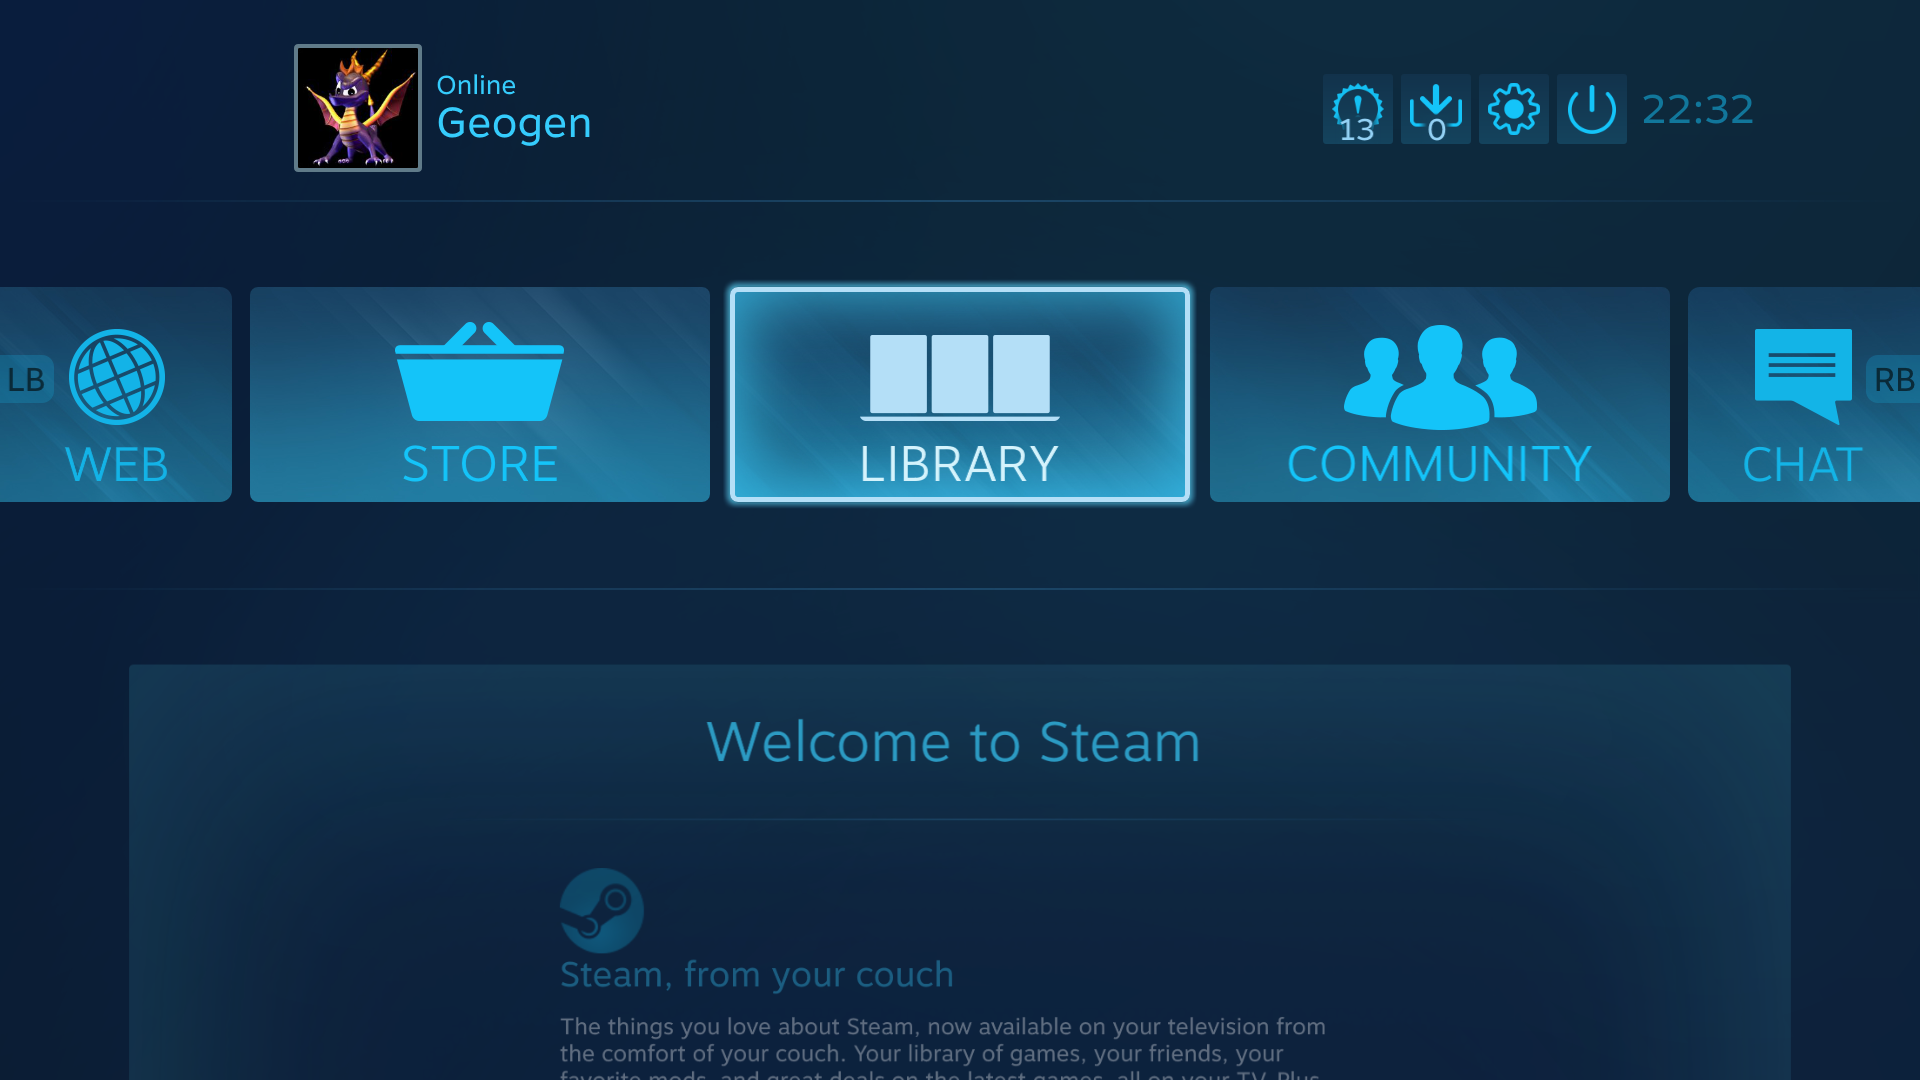
\includegraphics[width=16cm,height=9cm]{Screenshots/SteamScreenShots/SteamInBigPictureMode.png}
\caption{Big Picture Mode Enabled in the Steam Client}    
\end{figure}
This image shows how the Steam client is presented when in ``Big Picture Mode", which is a complete UI redesign suited for users who prefer using a controller over that of using mouse and keyboard.

\section{Figures associated with adding another user as a friend on Steam}

\begin{figure}[H]
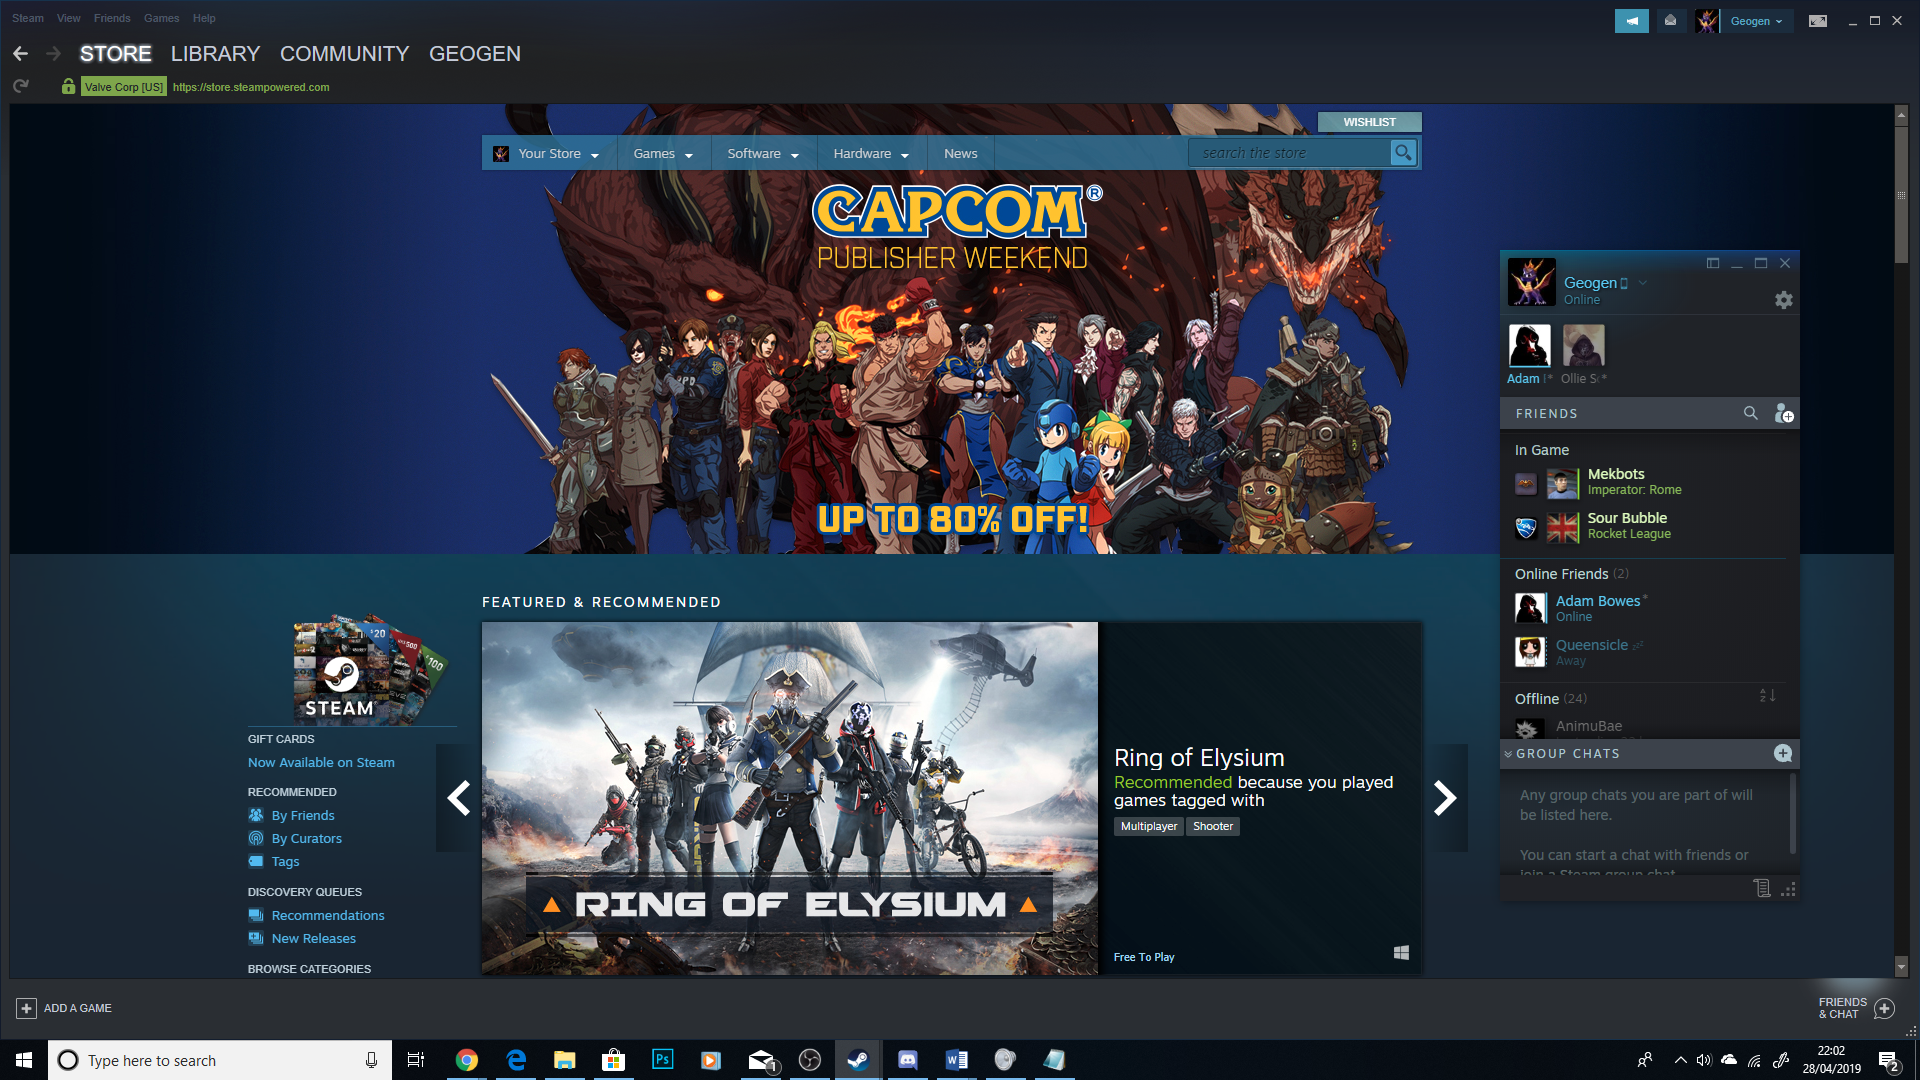
\includegraphics[width=16cm,height=9cm]{Screenshots/SteamScreenShots/friendsUI.png}
\caption{Friends UI element of the Steam client}    
\end{figure}

The Steam client has a convenient function to display the accounts friends. The user is pictured in this Figure and shows currently added friends, who are online and offline as well as what friends are playing.

\begin{figure}[H]
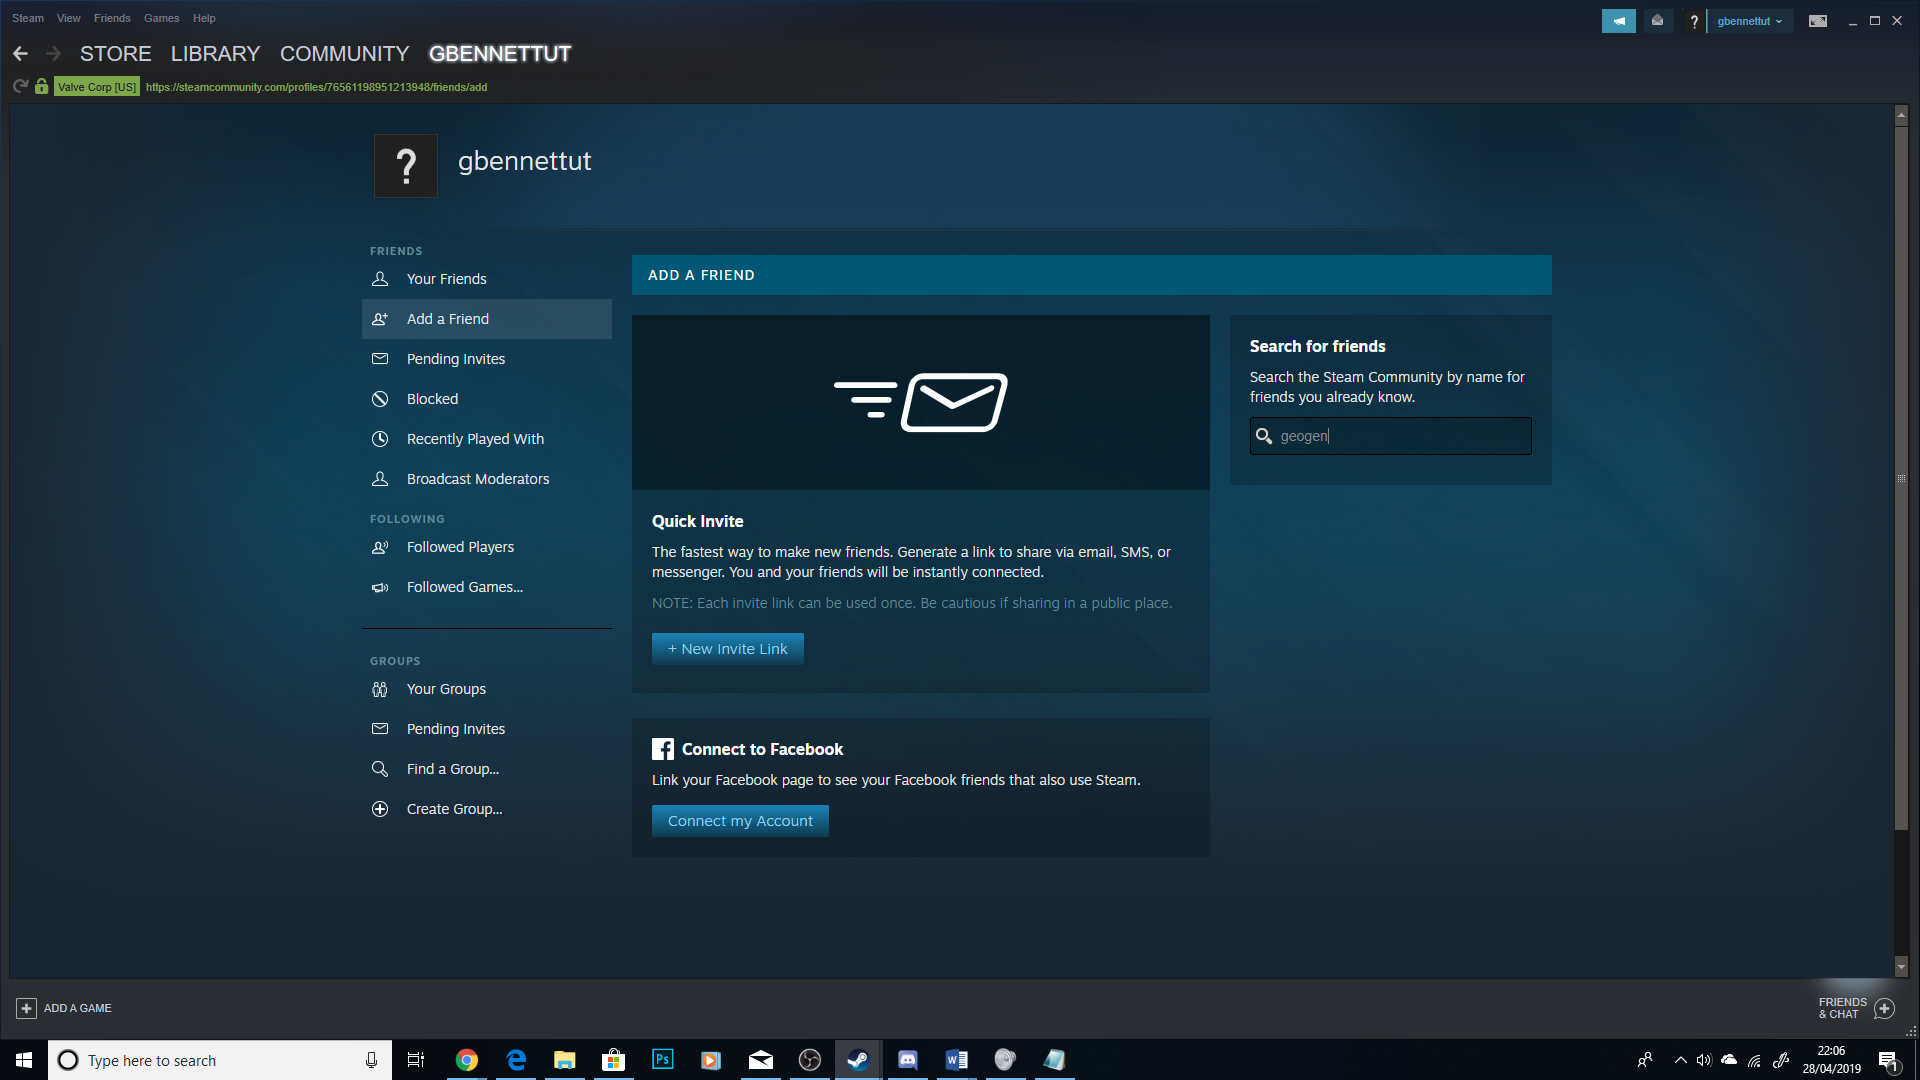
\includegraphics[width=16cm,height=9cm]{Screenshots/SteamScreenShots/searchforAFriend.png}
\caption{Searching for a fellow Steam user to add them as a friend}    
\end{figure}

I have clicked on the small icon of a user with a plus arrow in the previous Figure UI, and am now presented with the following screen, I will search for a user ``Geogen", in the appropriate location.

\begin{figure}[H]
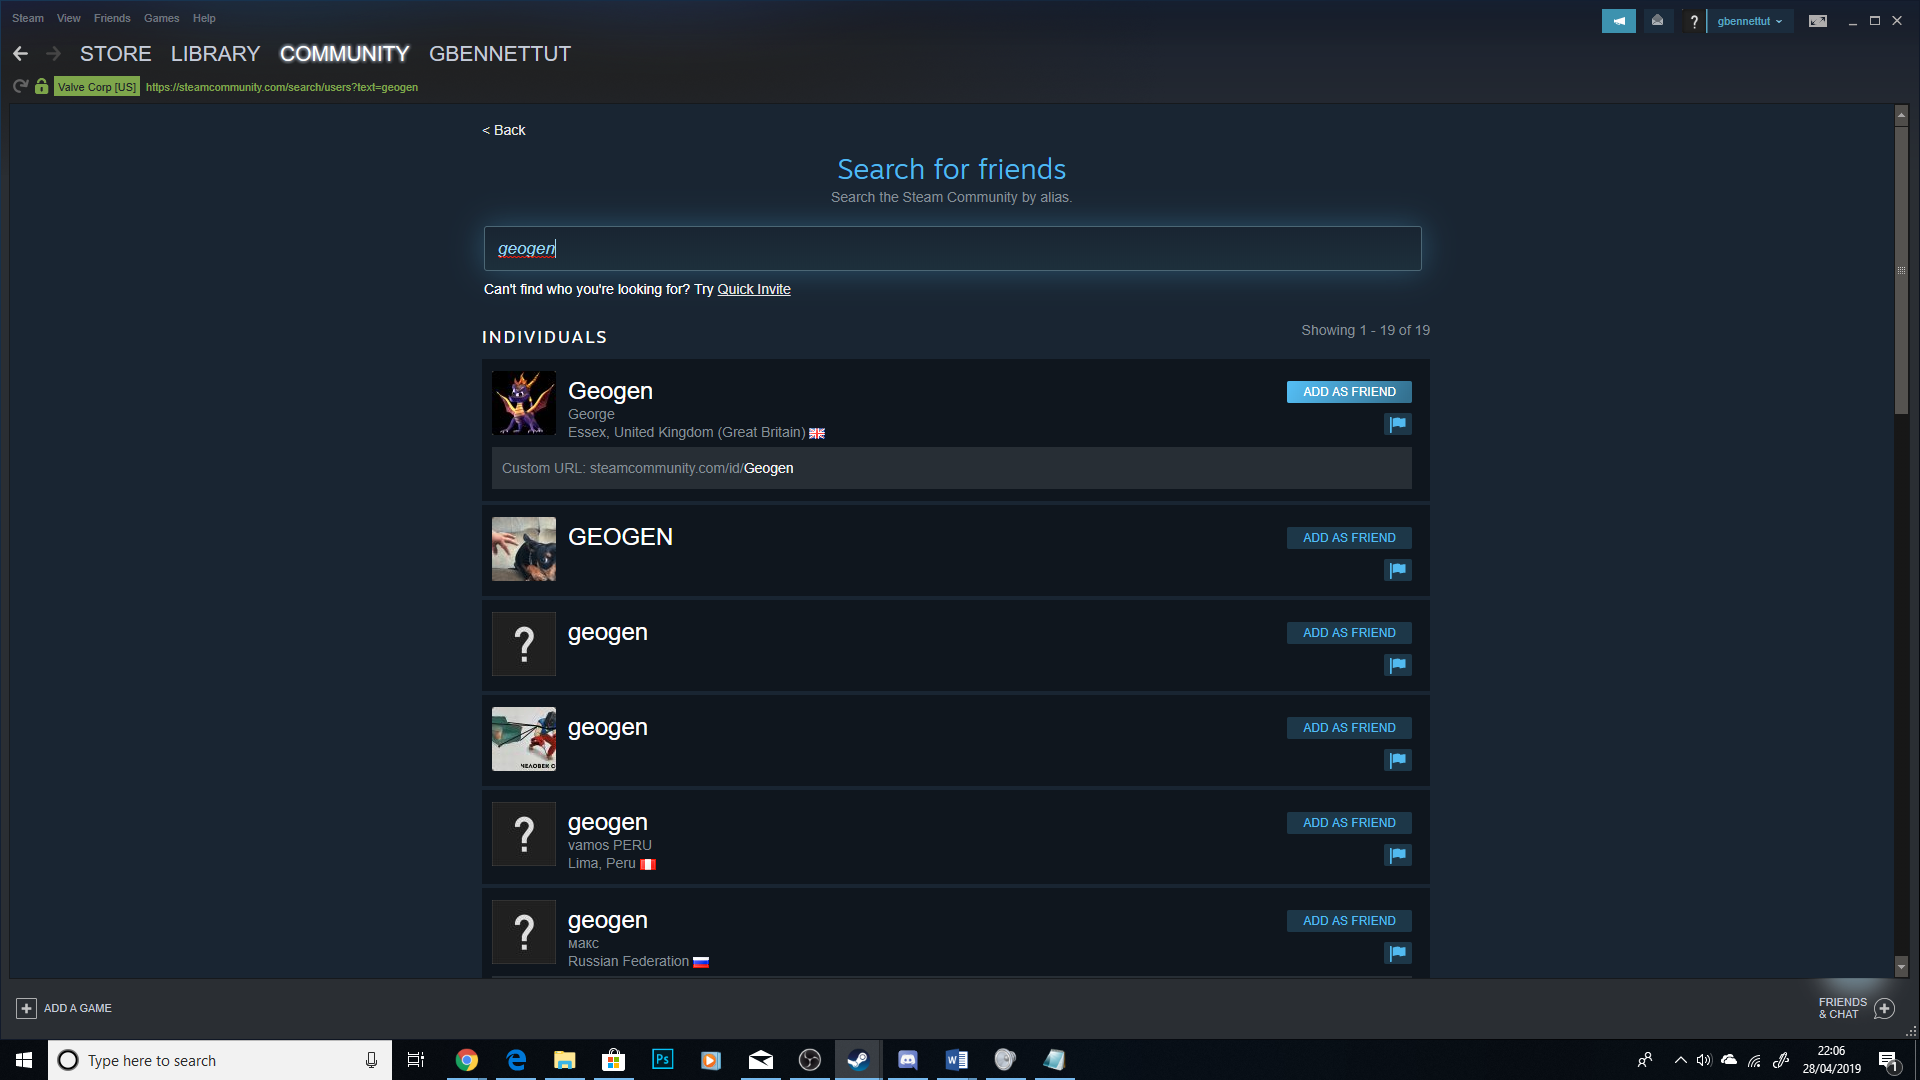
\includegraphics[width=16cm,height=9cm]{Screenshots/SteamScreenShots/friendRequestSent.png}
\caption{Sending a friend request to a desired user}    
\end{figure}

Following the previous Figure I have found a list of users with that name, the top user is the account I wish to add, so I have clicked the corresponding element (\textit{``ADD AS FRIEND"}) to send them a friend request.

